\chapter{Genomes and Some Simple Patterns}
\label{ch:genome}

The central dogma of molecular biology (Fig.~\ref{fig:g-central-dogma-genome}), the way we have also revealed in the Chapter~\ref{ch:intro-mol-biol}, explains how genetic information flows within living systems. In simple terms, it states that "DNA makes RNA makes protein." To elaborate, DNA contains the instructions for the sequence of amino acids in proteins. To create a protein, the information from the DNA—known as the protein-coding sequence—is first transcribed into messenger RNA (mRNA) and then translated into protein. The central dogma also emphasizes that this is the only direction in which information flows: the sequence of amino acids in proteins cannot be converted back into DNA.

\begin{figure}
  \centering{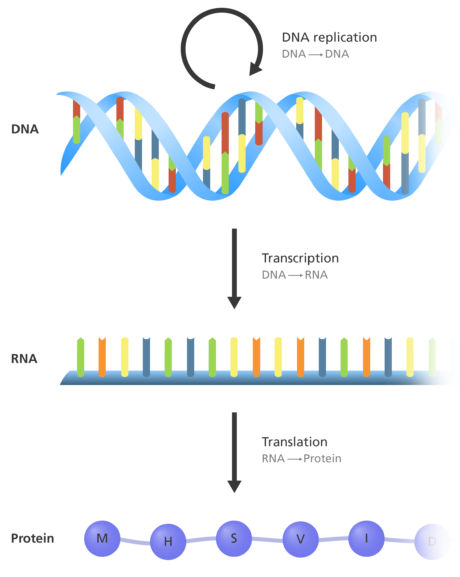
\includegraphics[width=0.5\textwidth]{figs/genome/central-dogma.png}}
  \caption[6pt]{The central dogma of molecular biology.}
  \label{fig:g-central-dogma-genome}
\end{figure}

At this stage, however, we should mention that biology is full of exceptions and surprises. The central dogma is a fundamental principle of molecular biology, but it is not the only way that genetic information is used in living systems. For example, some RNA molecules can have catalytic activity, and some proteins can interact with DNA to regulate gene expression. In addition, the central dogma does not account for the many ways that genetic information can be modified, such as by mutations, recombination, or epigenetic changes. Nevertheless, the central dogma provides a useful framework for understanding how genetic information is stored, transmitted, and used in living systems.

In this chapter, we will begin exploring genomes and DNA sequences. Our goal is to investigate whether these sequences are simply random arrangements of nucleotides or if there are recognizable patterns that can be identified, even without considering the genes. Understanding these patterns can provide valuable insights into the structure and function of DNA. We will focus on genes in the next chapter, where we will delve deeper into their roles and significance.

\section{Structure of Deoxyribonucleic Acid (DNA)}

Deoxyribonucleic acid (DNA) is a long molecule made of nucleotides, which consist of a sugar called deoxyribose, a phosphate group, and a nitrogenous base~\ref{fig:g-dna-detail}. There are four types of nucleotides: cytosine (C), guanine (G), adenine (A), and thymine (T). DNA has two strands that twist around each other to form a double helix. The strands are held together by weak hydrogen bonds, with adenine pairing with thymine, and cytosine pairing with guanine.

\begin{figure}
    \centering{
        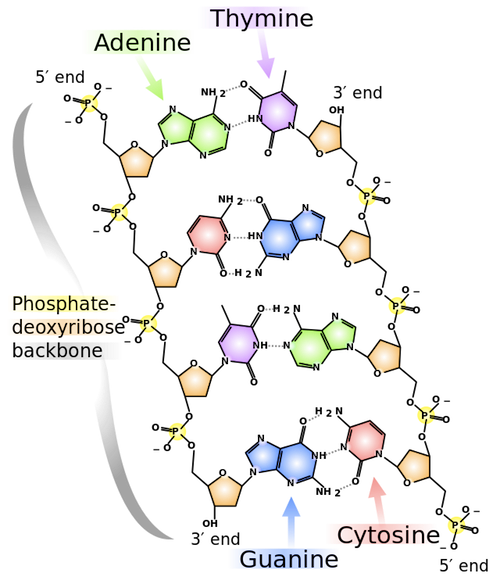
\includegraphics[width=0.6\textwidth]{figs/genome/dna-detail.png}
    }
    \caption[6pt]{The structure of DNA.}
    \label{fig:g-dna-detail}
  \end{figure}

Each strand has a repeating pattern of deoxyribose sugar and phosphate, forming a strong sugar-phosphate backbone. The nucleotides are attached to this backbone, with one nucleotide connected to each sugar group.

Because the two strands are complementary, one strand can always be used to determine the sequence of the other. Both strands carry the same genetic information, which is crucial for accurate DNA replication.

The difference in bond strength gives DNA a zipper-like quality. The weak hydrogen bonds make it easy to unzip the strands, while the strong covalent bonds in the backbone protect the structure from damage. This design provides both flexibility and stability, allowing DNA to perform its role in biological systems.

\section{Directionality of DNA Strands}

The two strands of DNA run in opposite directions, a property known as antiparallelism. To understand this concept, we need to examine the sugar group in the sugar-phosphate backbone. Chemists have established a system to number the carbon atoms in the sugar molecule, labeling them with ``prime'' notation, such as 1' (one-prime), 3' (three-prime), and so on. This helps organize the chemical structure and provides a clear reference for the orientation of the strands. Figure~\ref{fig:g-sugar} shows the atom numbering for the sugar group.

\begin{marginfigure}
  \centering{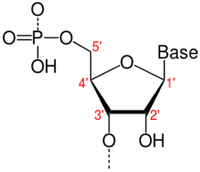
\includegraphics{figs/genome/sugar.png}}
  \caption[6pt]{Numbering of carbon atoms in a sugar group.}
  \label{fig:g-sugar}
\end{marginfigure}

In the DNA backbone, each sugar is linked to a phosphate group at its 5'-end (five-prime end) and to the next nucleotide through its 3'-end (three-prime end). The 5'-end of a DNA strand refers to the end with a free phosphate group attached to the 5' carbon of the sugar, while the 3'-end refers to the end with a free hydroxyl group (-OH) attached to the 3' carbon of the sugar.

This arrangement gives each DNA strand a directionality. One strand runs from the 5' end to the 3' end, while the complementary strand runs in the opposite direction, from 3' to 5'. This antiparallel structure is critical for many biological processes, such as DNA replication and transcription. The enzymes involved in these processes recognize the direction of the strands and ensure that each is copied or read correctly.

The 5' to 3' orientation also plays an essential role in the regulation of gene expression, as the directionality influences how various molecules interact with the DNA during cellular processes. Understanding this fundamental concept is key to grasping the mechanisms behind molecular biology and genetic information flow.

\section{Genome Size and Packaging}

The complete DNA sequence of an organism is called the genome. The genome represents the total genetic information contained within a cell, including the DNA in the nucleus and in any organelles. Interestingly, some organelles also contain DNA. In animals, this organelle is the mitochondrion, and in plants, it is the chloroplast. However, when we refer to the genome of eukaryotes, we usually mean the DNA in the nucleus. The genetic material in the mitochondria is referred to as the mitochondrial genome.

In the nucleus, DNA is typically not a single continuous molecule but is divided into segments and organized into chromosomes. For example, humans have 23 pairs of chromosomes. However, we won’t focus on chromosomes just yet, so there’s no need to worry about them for the next few lectures.

This structure allows the genome to be efficiently packaged and organized, facilitating processes like cell division and gene expression. The size of the genome can vary greatly between species, but it always contains all the information necessary for the development, functioning, and reproduction of the organism.


So what is the total length of the DNA sequence? It depends on the organism, as shown in Figure~\ref{fig:g-genome-size}. Prokaryotes, such as bacteria, have the shortest genomes. We measure DNA length in base pairs (bp), which refers to two nucleobases bound together by hydrogen bonds. Simply put, one base pair consists of one nucleotide on each strand of the DNA. The total number of nucleotides on one strand determines the size (or length) of the genome.

\begin{figure}
    \centering{
        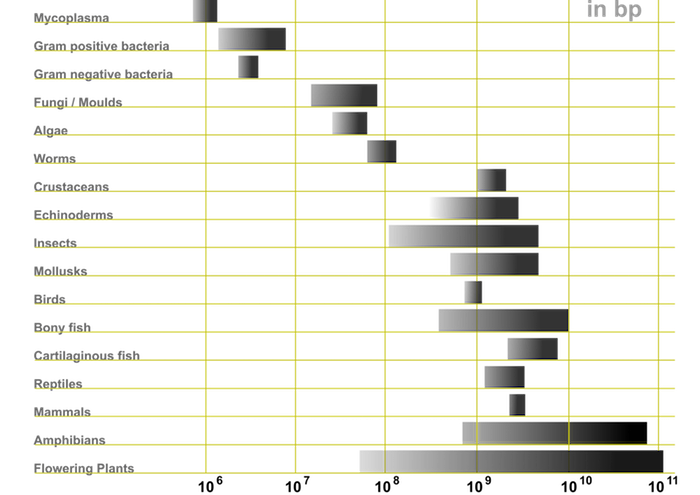
\includegraphics[width=0.95\textwidth]{figs/genome/genome-size.png}
    }
    \caption[6pt]{Genome sizes of various organisms.}
    \label{fig:g-genome-size}
  \end{figure}

Bacterial genomes typically range from 0.5 to 13 megabase pairs (Mbp), where one Mbp equals one million (10\textsuperscript{6}) base pairs. The abbreviation "Mb" is often used to represent megabase pairs.

Eukaryotic genomes are much larger, ranging from 8 Mb to 670 gigabase pairs (Gb), with one Gb equaling one billion (10\textsuperscript{9}) base pairs. In contrast, viruses have much smaller genomes, ranging in size from 5 to 50 kilobase pairs (kb), where one kb equals one thousand (10\textsuperscript{3}) base pairs.

And what about us, humans? Our genome contains about 3,200 Mb, or 3.2 Gb. To put that in perspective, the first Harry Potter book, Harry Potter and the Philosopher's Stone, contains 76,944 words. With the average English word being just over 5 letters long, the book contains approximately 384,720 letters. If we represented each nucleotide in the human genome as a single letter, we would need the equivalent of 8,300 Philosopher's Stone books to write out the human genome.

To visualize this further, my version of Harry Potter and the Philosopher's Stone is about 2 cm thick. If we stacked 8,300 of these books, one on top of another, the stack would reach a height of around 166 meters.

If we could stretch out the DNA from a single human cell, it would form a very thin thread about 2 meters long. Despite this length, the DNA is tightly packed into the cell's nucleus, which is only about 5-10 micrometers in diameter. This incredible compaction is made possible because the DNA is wrapped around proteins called histones, forming a structure known as chromatin. This efficient organization allows the large amount of DNA to fit neatly inside the small space of the cell nucleus.

\section{Exploring Viral Genomes: Lambda Phage as a Case Study}

Let us start small—with a virus. Lambda phage is a bacterial virus that infects and destroys \textit{Escherichia coli} bacteria. This virus, like many others, has its genome fully sequenced and available for research. You may have noticed the scientific name \textit{Escherichia coli}. These names follow binomial nomenclature, a system using Latin names composed of a genus and species. For example, humans are classified as \textit{Homo sapiens}.

Now, back to Lambda phage. One of the sources for its genome information is GenBank\footnote{\url{https://www.ncbi.nlm.nih.gov/genbank}}, a sequence database maintained by The National Center for Biotechnology Information (NCBI). GenBank hosts a page dedicated to the Lambda phage genome\footnote{\url{https://www.ncbi.nlm.nih.gov/nuccore/NC_001416.1}}).

The GeneBank's page contains several key pieces of information. It includes data about the scientists and research groups that sequenced and published the genome, as well as a detailed description of the genome’s structure. The page also lists the specific genes encoded within the genome and their functions. Finally, at the bottom of the page, you'll find the complete DNA sequence of Lambda phage, represented as a string of nucleotides (A, T, C, G). This sequence is what we are most interested in for bioinformatics analysis.

If you are curious about the meaning of the various fields and terms on this page, you can refer to the Sample GenBank Record page\footnote{\url{https://www.ncbi.nlm.nih.gov/genbank/samplerecord}}). Clicking on any of the terms will provide an explanation of their significance.

While all this information is available through the web page, we are more focused on how to access it programmatically. This allows us to automate the retrieval of genomic data for further analysis and manipulation, which is essential for large-scale bioinformatics tasks. Let's see how we can retrieve the Lambda phage genome sequence using Python:

\vspace*{3mm}
\begin{lstlisting}
>>> from Bio import Entrez, SeqIO
>>> Entrez.email = "blaz.zupan@fri.uni-lj.si"
>>> with Entrez.efetch(db="nucleotide", 
>>>   id="NC_001416", rettype="gb") as handle:
>>>    data = SeqIO.read(handle, "genbank")
>>> len(data.seq)
48502
>>> data.seq[:10]
Seq('GGGCGGCGAC')
\end{lstlisting}

The genome of {\em Lambda phage} contains 48,502 base pairs. We have the sequence for only one strand; the other strand is simply its reverse complement. The genome starts with three guanine nucleotides (G). Which nucleotides are the most prevalent in the {\em Lambda phage} genome?

\vspace*{3mm}
\begin{lstlisting}
>>> from collections import Counter
>>> Counter(data)
Counter({'G': 12820, 'A': 12334, 'T': 11986, 'C': 11362})
\end{lstlisting}

The most prevalent nucleotide in the {\em Lambda phage} genome is guanine (G), followed by adenine (A), thymine (T), and cytosine (C). The genome is well balanced in terms of nucleutide frequency. The question is if this is so for all the genomes, and since we have the tools, we can check this some other organism. 

Let's do this for the bacteria {\em Mycoplasma genitalium}, a tiny bacterium that causes sexually transmitted infections. It can lead to problems like inflammation in the urinary tract (in men) or the cervix and pelvic area (in women). For bioinformatics, this bacterium is interesting because it has one of the smallest genomes of all free-living organisms.

\vspace*{3mm}
\begin{lstlisting}
>>> from Bio import Entrez, SeqIO
>>> Entrez.email = "blaz.zupan@fri.uni-lj.si"
>>> with Entrez.efetch(db="nucleotide", 
>>>   id="NC_000908.2", rettype="gb") as handle:
>>>    data = SeqIO.read(handle, "genbank")
>>> data.description
'NC_000908.2 Mycoplasma genitalium G37, complete sequence'
>>> len(data.seq)
580076
>>> Counter(data)
Counter({'A': 200544, 'T': 195711, 'G': 92306, 'C': 91515})
>>> n = sum(counts.values())
>>> for c in counts.keys():
>>>   print(f"{c}: {counts[c]:,} ({counts[c]/n:.1%})")
T: 195695 (33.7%)
A: 200543 (34.6%)
G: 92312 (15.9%)
C: 91524 (15.8%)
\end{lstlisting}

The genome of {\em M. genitalium} is not balanced. In fact, the adenine and thymine are most prevalent and interestingly their frequency is almost equal. And so the frequency of cytosine and guanine is also almost equal. This is a common feature of many genomes, where the adenine-thymine and cytosine-guanine pairs are balanced. This balance is important for the stability of the DNA double helix, as the adenine-thymine and cytosine-guanine pairs have different numbers of hydrogen bonds. The balance of these pairs helps maintain the stability of the DNA structure, and it was evolutionarily selected to ensure the integrity of the genetic information.

Of course, at this stage, we could test prevalency of balance betwee A-T and C-G pairs for other organisms. Say, in human. The smallest human chromosome is Chromosome 21. Despite its small size, it plays a critical role in development and health. For example, having an extra copy of Chromosome 21 leads to Down syndrome. Fetching the sequence of this chromosome, even though it is not the smallest, takes time, so it may help if we reorganize our code so that we can save the data locally for any rerun of the analysis.

\vspace*{3mm}
\begin{lstlisting}
  import os.path
  from Bio import Entrez, SeqIO
  from collections import Counter
  
  Entrez.email = "blaz.zupan@fri.uni-lj.si"
  
  organism_id = {
      "Hs_21": "NC_000021.9", # Homo sapiens genomic DNA
      "Pl": "NC_001416.1",  # Phage lambda
      "Mt": "AL123456.3",  # Mycobacterium tuberculosis
      "Mg": "NC_000908.2",  # Mycoplasma genitalium
      "Ec": "NC_000913",  # E coli
  }
  organism = "Hs_21"
  
  filename = f"data/{organism}.fasta"
  if os.path.exists(filename):
      print(f"Loading {organism} sequence from local file.")
      data = SeqIO.read(filename, "fasta")
  else:
      print(f"Fetching {organism} ...")
      with Entrez.efetch(
          db="nucleotide",
          id=organism_id[organism],
          rettype="gbwithparts",
          retmode="text"
      ) as handle:
          data = SeqIO.read(handle, format="genbank")
  
      print("Storing ...")
      with open("data/%s.fasta" % organism, "w") as f:
           SeqIO.write([data], f, "fasta")
  
  print(f"Genom eID: {data.id}")
  print(f"Description:\n{data.description}")
  print(f"Genome size: {len(data.seq):,}")
  
  counts = Counter(str(data.seq))
  n = sum(counts.values())
  for c in counts.keys():
      print(f"{c}: {counts[c]:,} ({counts[c]/n:.1%})")
\end{lstlisting}

The code above checks if the sequence of the organism is already stored locally. If it is, it loads the sequence from the file. If not, it fetches the sequence from the NCBI database and stores it locally. This way, we can avoid repeatedly downloading the same data, which can be time-consuming and inefficient. Running the code we get:

\vspace*{3mm}
\begin{lstlisting}
Loading Hs_21 sequence from local file.
Genom eID: NC_000021.9
Description: 
NC_000021.9 Homo sapiens chromosome 21, GRCh38.p14 Primary Assembly
Genome size: 46,709,983
N: 6,621,361 (14.2%)
G: 8,226,381 (17.6%)
A: 11,820,664 (25.3%)
T: 11,856,330 (25.4%)
C: 8,185,244 (17.5%)
M: 2 (0.0%)
R: 1 (0.0%)
\end{lstlisting}

Great, A-T and G-C pairs are balanced once more. But what about the other letters? In genome sequences, characters other than A (Adenine), T (Thymine), G (Guanine), and C (Cytosine) indicate ambiguous nucleotide bases or unique cases. These additional symbols follow the IUPAC (International Union of Pure and Applied Chemistry) nucleotide code:

\begin{itemize}
\item N: any nucleotide (A, T, G, or C), the specific base is unknown,
\item M: either A (Adenine) or C (Cytosine). M stands for ``amino'', because both adenine and cytosine have an amino group attached to their structures.
\item R: either A (Adenine) or G (Guanine). R stands for ``purine'', because both adenine and guanine are purines, which are a class of nitrogenous bases with a two-ring structure.
\end{itemize}

\section*{Accession Numbers}

You may notice that in the code so far we have used NCBI's accession numbers, that is, unique identifiers assigned to specific sequences in the National Center for Biotechnology Information (NCBI) databases. For example, the NC\_000021.9 accession number corresponds to Chromosome 21 of {\em Homo sapiens}, and AL123456.3 corresponds to the genome of {\em Mycobacterium tuberculosis}, the bacterium responsible for tuberculosis.

Accession numbers allow researchers to reference and access genome sequences, genes, or proteins easily. Typically, accession numbers are assigned when a new sequence is submitted to NCBI as part of a genome or protein record. To obtain them, researchers sequence the DNA, validate it, and submit the data through the NCBI submission tools like GenBank. To find an accession number, one can search for an organism, gene, or sequence of interest using NCBI’s search tools, such as Entrez, which will return the corresponding accession number for that specific dataset. For a start, one may also query any of the well-trained large language models, such as GPT-3, to find the accession number for a specific organism or gene.

\section*{Time for Some Formalism}
To describe a DNA sequence, we will use lists of symbols from an alphabet $\mathcal{N} = \{A, C, T, G\}$. We will represent sequences with vectors and denote them with symbols like $\vec{x}$, $\vec{s}$, and $\vec{t}$. Most often, we will be lazy and omit the arrow, using symbols like $x$, $s$, and $t$ for sequences.

Consider now a DNA sequence $x$. This is a finite string from the alphabet $\mathcal{N}$, such that $x = x_1x_2x_3 \dots x_n$, where $x_i$ is an element of the string and $x_i \in \mathcal{N}$.

\section*{Multinomial Model of a Sequence}

The simplest (and the least useful) model of a sequence is a multinomial model. This model simply contains the probabilities with which each of the nucleotides appears in the sequence. The model assumes that nucleotides are independently and identically distributed. In statistics, this assumption is abbreviated as i.i.d. "Independently" here means that the probability of encountering a symbol in a sequence does not depend on the sequence position or any of the neighbors in the sequence. Intuition suggests that this may not be the case in DNA, but the multinomial model can still provide a foundation for reasoning about the sequence, particularly in understanding how sequences violate the i.i.d. property.

The multinomial model of a DNA sequence is defined as $\vec{p} = (p_A, p_C, p_T, p_G)$, where $p_z = p(x_i = z)$ and $\sum_{z \in \{A, C, T, G\}} p_z = 1$.

Given a multinomial model, the probability of a sequence is
\[
P(x) = \prod_{i=1}^{n} p(x_i)
\]
Do you think this probability will be large, small, or perhaps very, very small? Why?

We have already estimated the parameters of the multinomial model in the code a few pages back, and used relative frequency for this task. Just to write it formally, the relative frequency of a nucleotide $z$ in a sequence $x$ is:
\[
\hat{p}_z = \frac{{\rm count}(z, x)}{n}
\]
where ${\rm count}(z, x)$ is the number of occurrences of nucleotide $z$ in the sequence $x$ and $n$ is the length of the sequence.

\section*{Finding Unusual DNA Words}

More than the probabilities of individual nucleotides, we might be interested in the probabilities of short subsequences of length $k$. Here, in this section, we will consider only dinucleotides, which are subsequences of length $k=2$. For example, we may want to observe whether a subsequence CG appears more often than would be expected by chance. 

By chance, using our multinomial model, the probability that a random nucleotide pair would form the combination C and G (i.e., a subsequence CG) is equal to $p_C \times p_G$. That’s straightforward. So what, then, is the probability of CG that we can estimate from the actual genome? We observe all the dinucleotides (there are $n-1$ of them) and count how many of them are equal to CG. Thus, we estimate this probability as $\frac{N_{CG}}{n-1}$, where $N_{CG}$ is the number of occurrences of the dinucleotide CG in the sequence $x$.

Next, we can compute the odds ratio, which is the ratio between the observed probability and the expected probability of the dinucleotide, where the expected probability comes from the multinomial model constructed under the assumption of i.i.d., meaning no order in the genome:
\[
{\rm odds ratio} = \frac{N_{CG}/(n-1)}{p_C \times p_G}
\]

Often, instead of the odds ratio, we report the log odds ratio, as it provides a symmetrical measure of surprise centered at 0. The subsequences that appear more often than expected have positive log odds ratios, while those that appear less often than expected have negative log odds ratios.

Time to implement this in code. We start with the generator of dinucleotides:

\vspace*{3mm}
\begin{lstlisting}
def tuple_walk(s, k=2):
  """Generate all k-tuples from sequence s."""
  for i in range(len(s) - (k-1)):
    yield s[i:i+k]

def count_tuple(s, w):
  """Count words w in sequence s."""
  return sum(1 for ss in tuple_walk(s, len(w)) if ss == w)
\end{lstlisting}

Let's use these functions on a short sequence, just to check it out:

\vspace*{3mm}
\begin{lstlisting}
>>> s = "ACCTAGGCT"
>>> list(tuple_walk(s))
['AC', 'CC', 'CT', 'TA', 'AG', 'GG', 'GC', 'CT']
>>> count_tuple(s, "CT")
2
\end{lstlisting}

Fine. This seems to work. Now we can implement the odds ratio computation, and put all the code together to analyze the H. sapiens chromosome 21:

\vspace*{3mm}
\begin{lstlisting}
from Bio import SeqIO
from collections import Counter
import math

def tuple_walk(s, k=2):
    """Generate subsequences of length k."""
    for i in range(len(s)-1):
        yield s[i:i+k]

def count_tuple(s, w):
    """Count words w in sequence s."""
    return sum(1 for ss in tuple_walk(s, len(w)) if ss == w)

organism = "Hs_21"

filename = f"data/{organism}.fasta"
s = str(SeqIO.read(filename, "fasta").seq)

subsequence = "CG"
count = count_tuple(s, subsequence)
print(f"Count of {subsequence} on original sequence: {count:,}")

n = len(s)
p_nucleotide = {k: v/n for k, v in Counter(s).items()}
p = math.prod(p_nucleotide[x] for x in subsequence)
print(f"Expected: {int((p * n)):,}")
odds = (count / n) / p
print(f"Odds ratio: {odds:.2f}")
print(f"Log odds ratio: {math.log(odds):.2f}")
\end{lstlisting}

Running the code we get:

\vspace*{3mm}
\begin{lstlisting}
Count of CG on original sequence: 462,299
Expected: 1,441,553
Odds ratio: 0.32
Log odds ratio: -1.14
\end{lstlisting}

The dinucleotide \textbf{CG} appears less frequently than expected by chance. The log odds ratio is negative, indicating that the observed frequency of CG is lower than the expected frequency under the multinomial model. This is not surprising, as the dinucleotide CG is known to be less common in the human genome. However, CG dinucleotides are often concentrated in specific regions called \textbf{CpG islands}, which are associated with gene regulation and epigenetic modifications.

In the abbreviation ``CpG,'' the \textbf{p} refers to the phosphate group that links the cytosine (C) and guanine (G) nucleotides in the DNA backbone. \textbf{CpG islands} are typically found near gene promoters and play a crucial role in regulating gene expression (more on this in the next chapters).

\begin{marginfigure}
  \centering{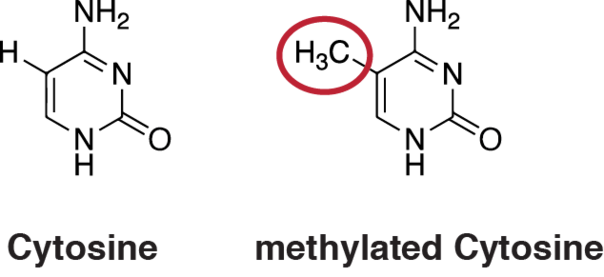
\includegraphics{figs/genome/dna-methylation.png}}
  \caption[6pt]{DNA methylation.}
  \label{fig:g-dna-methylation}
\end{marginfigure}

The lower frequency of CG dinucleotides in the genome is primarily due to the methylation of cytosine, which converts it to 5-methylcytosine. Over evolutionary time, methylated cytosines tend to mutate into thymines (T) due to a process called deamination. This mutation results in a gradual loss of CG dinucleotides from the genome, leading to fewer CpG islands than might be expected by chance.

This reduction in CG content may have provided evolutionary benefits\sidenote{The discovery of DNA methylation in the 1940s by Rollin Hotchkiss gave rise to the field of epigenetics, which studies changes in gene expression without altering the DNA sequence. These changes, such as the methylation of cytosine in CpG dinucleotides, can silence or reduce gene activity. Importantly, epigenetic modifications can be inherited during cell division and, in some cases, passed from one generation to the next, meaning environmental factors can influence not only an individual’s gene expression but also potentially impact their offspring.}. Methylation and subsequent mutations likely played a role in genome defense mechanisms, such as \textit{silencing transposable elements} (DNA sequences that can move around in the genome) to prevent them from disrupting functional genes. Additionally, selective pressure may have favored fewer CpG dinucleotides outside of CpG islands to reduce unnecessary mutations that could affect essential gene regulation mechanisms.

Just one more note about methylation: the mechanism that retains methylation during DNA replication is called {\bf maintenance methylation}. This process is carried out by an enzyme called {\bf DNA methyltransferase 1 (DNMT1)}. When DNA is replicated, the new strand is synthesized without methylation marks. DNMT1 recognizes the hemimethylated DNA (where the parent strand is methylated and the newly synthesized strand is not) and adds methyl groups to the corresponding sites on the new strand. This ensures that the methylation pattern is preserved across cell divisions, maintaining the epigenetic state of the genome.

Other than \textbf{CpG}, the dinucleotides \textbf{TpA (TA)} and \textbf{CpA (CA)} are also of interest in genomic studies, each for different reasons:

\begin{itemize}
    \item \textbf{TpA (TA)}: This dinucleotide is often underrepresented in genomic sequences, likely due to its association with instability in the DNA double helix. TA sequences can form weak bonds, making them more prone to mutations and breakage. This dinucleotide also plays a role in certain regulatory regions like promoters and is found in repetitive elements.
    
    \item \textbf{CpA (CA)}: CA dinucleotides are frequently found in regions of active gene expression and are often involved in alternative splicing. Methylation of CpA is also emerging as a topic of interest, particularly in non-CpG methylation, which is being linked to developmental and tissue-specific gene regulation.
\end{itemize}

Both of these dinucleotides, along with others, contribute to the broader understanding of DNA sequence evolution, mutability, and regulation of gene expression.

\section{Where to Go from Here}

This chapter offers just a glimpse into the world of genomes and DNA sequences. We continue with further exploration of the genome sequnces in our next chapter, where we focus on finding genes.
